% iaus2esa.tex -- sample pages for Proceedings IAU Symposium document class
% (based on v1.0 cca2esam.tex)
% v1.04 released 17 May 2004 by TechBooks
%% small changes and additions made by KAvdH/IAU 4 June 2004
% Copyright (2004) International Astronomical Union

\NeedsTeXFormat{LaTeX2e}

\documentclass{iau}
\usepackage{graphicx}
\usepackage{caption}
\usepackage{hyperref}

\title[Asteroids in LSST] %% give here short title %%
{Asteroid Discovery and Characterization with the Large Synoptic Survey Telescope}

\author[R. Lynne Jones, Mario Juric]   %% give here short author list %%
{R. Lynne Jones$^1$, Mario Juri\'{c}$^2$, 
%%  \thanks{Present address: Department of Astronomy, University of
%%  Washington, Seattle, USA},
 \and \v{Z}eljko Ivezi\'{c} $^3$}

\affiliation{$^1$University of Washington\\ email: {\tt ljones@astro.washington.edu} \\[\affilskip]
$^2$University of Washington \\email: {\tt mjuric@astro.astro.washington.edu}
$^3$University of Washington \\email: {\tt ivezic@astro.astro.washington.edu}}

\pubyear{2015}
\volume{318}  %% insert here IAU Symposium No.
\setcounter{page}{1}
\jname{Asteroids: New Observations, New Models}
\editors{Steve Chesley, Alessandro Morbidelli, Robert Jedicke \&
  Davide Farnocchia eds.}
\begin{document}

\maketitle

\begin{abstract}
The Large Synoptic Survey Telescope (LSST) will be a ground-based,
optical, all-sky, rapid cadence survey project with tremendous
potential for discovering and characterizing asteroids.

With LSST's large 6.5m diameter primary mirror, a wide 9.6 square
degree field of view 3.2 Gigapixel camera, and rapid observational
cadence, LSST will discover more than 5 million asteroids over its ten
year survey lifetime. With a single visit limiting magnitude of 24.5
in $r$ band, LSST will be able to detect asteroids in the Main Belt
down to sub-kilometer sizes.  The current strawman for the LSST survey
strategy is to obtain two visits (each `visit' being a pair of
back-to-back 15s exposures) per field, separated by about 30 minutes,
covering the entire visible sky every 3-4 days throughout the
observing season, for ten years.

The catalogs generated by LSST will increase the known number of small
bodies in the Solar System by a factor of 10-100 times, among all
populations. The median number of observations for Main Belt asteroids
will be on the order of 200-300, with Near Earth Objects receiving a
median of 90 observations. These observations will be spread among
$ugrizy$ bandpasses, providing photometric colors and the allowing
sparse lightcurve inversion to determine rotation periods, spin axes, and shape information.

These catalogs will be created using automated detection software, the
LSST Moving Object Processing System (MOPS), that will take advantage
of the carefully characterized LSST optical system, cosmetically
clean camera, and recent improvements in difference imaging. Tests
with the prototype MOPS software indicate that linking detections (and thus
`discovery') will be possible at LSST depths with our working
model for the survey strategy, but evaluation of MOPS and improvements
in the survey strategy will continue. All data productsand software created by
LSST will be publicly available.
\keywords{Keyword1, keyword2, keyword3, etc.}
%% add here a maximum of 10 keywords, to be taken form the file <Keywords.txt>
\end{abstract}

\firstsection % if your document starts with a section,
                     % remove some space above using this command.

\section{Introduction}

The Large Synoptic Survey Telescope (LSST) is a next-generation survey
project, coupling a world-class telescope facility with cutting-edge
data management software and calibration efforts. Its primary science
drivers are to constrain dark matter and dark energy, to map the Milky
Way and Local Volume, to catalog the Solar System, and to explore
the transient optical sky. The catalogs generated by LSST during its
ten years of operation will enable a multitude of science
investigations beyond these primary science drivers, many of which are
explored in the LSST Science Book (ref).

The inventory of the Solar System is one of the primary science
drivers for LSST; fulfilling this science goal will include
discovering millions of minor planets, increasing the number of known
objects in every small body population by a factor of 10 to 100 above
current levels. Almost all of these objects will receive large numbers
($>100$) of observations, over a long time span (several years) and with
extremely accurate astrometry (10mas errors), resulting in highly
accurate orbits suitable for a wide range of theoretical studies or
for targeted follow up observations for specific purposes (such as
spectroscopy or occultation studies).

These large number of observations will also provide the basis for
sparse lightcurve inversion, which requires at least 100 observations
over a range of phase angles (ref). It will be possible to determine
the spin states and shapes for thousands of Main belt
asteroids. Frequent observations, spread among a wide range of times
and at variety of different points along each object's orbit, are also
ideal for detecting activity, either collisionally-induced activity or
surface activity induced by volatile outgassing (ref).

Each object will obtain observations in different filters, primarily $g$,
$r$, $i$ and $z$ but also $u$ and $y$, with photometric calibration of
each measurement accurate to 10mmags (lsst photoref). This will enable study of the
composition of these objects (ref). Adding color information also
provides statistical constraints on the albedos of the objects,
allowing a tighter estimate of the diameters and thus size
distribution of the population. With combined color and orbital
information, identification of collisional families becomes more
robust. Table \ref{table1} provides a summary of the expected number
of objects in each population, as well as their typical arc length and
number of observations.

\begin{table}
\begin{center}
\caption{Summary of small body populations observed with LSST}
\label{table1}
 {\scriptsize
  \begin{tabular}{|l|c|c|c|c|}\hline
Population & Currently known$^1$ &  LSST discoveries$^2$ &
Num. of obervations$^3$
    & Arc length (years)$^3$ \\ \hline
Near Earth Objects \\(NEOs) & 12,832 & 100,000 & (H$\leq$20) 90 & 7.0 \\
    \hline
Main Belt Asteroids \\(MBAs) & 636,499 & 5,500,000 & (H$\leq$19) 200 &
                                                                     8.5
    \\ \hline
Jupiter Trojans & 6,387 & 280,000 & (H$\leq$16) 300 & 8.7 \\ \hline
TransNeptunian and \\ Scattered Disk Objects \\ (TNOs and SDOs) & 1,921 &
                                                                    40,000
                                                                          &
                                                                            (H$\leq$6)
                                                                            450
    & 8.5 \\ \hline
 \end{tabular}
  }
 \end{center}
\vspace{1mm}
 \scriptsize{
 {\it Notes:}\\
  $^1$As reported by the MPC (May 2015).
  $^2$Expected at the end of LSST's ten years of operations.
  $^3$Median number of observations and observational arc length for the brightest objects near
  100\% completeness (as indicated). }
\end{table}

Construction for LSST is ongoing, with first light scheduled for 2020,
a scientific commissioning program following in the next year, and the
start of survey operations in 2022. Details of LSST operations are
currently being examined. In particular, the survey strategy continue
to be analyzed up to and during operations in order to maximize the
science return across the wide variety of goals for LSST. In this
proceedings, we will describe the planned LSST configuration, and
expected LSST performance in discovering and characterizing Near Earth
Objects (NEOs) and Main Belt asteroids (MBAs), then present software
tools that can aid the planetary astronomy community in extending
this analysis.

%sci book ref
%sparse lightcurve ref (with N of obs)
%activity refs
%occultation ref (with N of obs?)
%composition ref
%WISE albedo ref
%collisional family ref

\section{The LSST telescope}

The primary science goals for LSST drive the design of the telescope
and camera. The final design includes an optical telescope with
$ugrizy$ filters. The primary mirror for the
telescope is 8.4m in diameter; the effective diameter is 6.7m after
account for obscuration and vignetting. The telescope has a fast f/1.2
focal ratio; together with the 3.2 Gigapixel camera, this provides a
9.6 square degree field of view (with 0.2''/pixel platescale). The
fill factor of the camera is 90\%, counting active silicon within a
$3.5^\circ$ diameter circle inscribed in the field
of view; the fill factor counting only chip gaps but over the entire
(non-circular) focal plane is slightly higher, but similar. See Figure \ref{focalplane} for
an illustration of the focal plane.


The current plan is that LSST will obtain pairs of short (15 second)
exposures, combining these into an equivalent 30 second `visit' to
combat cosmic rays. In order to maintain a high duty cycle, the
overhead for each visit is short: 2 second readout per exposure and a
5 second slew/settle time between visits (for short slews).

With the information above, combined with weather information from the
Cerro Pachon site (such as the expected atmospheric IQ and sky
brightness) and system engineering data on the expected throughput
response curves, we can calculate the fiducial five sigma limiting
depths for LSST. Based on records from an on-site monitoring system,
the median atmospheric IQ is 0.66, 0.61, 0.56, 0.53, 0.50, 0.48
arcseconds in our $ugrizy$ bandpasses, respectively. The telescope
hardware is expected to contribute an additional 0.4''. In dark sky,
at zenith, the sky brightness is expected to be 23.0, 22.2, 21.2,
20.5, 19.6, and 18.6 mags/sq arcsecond in $ugrizy$, respectively. This
is based on dark sky spectra obtained from other sites, but verified
by broad band sky brightness measurements at Cerro Pachon.

System engineering continually updates the expected throughput curves,
based on updated data from prototype sensors and the expected performance of
the mirrors and filters and lenses, including broadband coatings and
loss estimates due to condensation and contamination. The current
performance estimates are available in a github repository, at
\url{http://github.com/lsst-pst/syseng_throughputs}.  Using these
throughput curves and the information above, we can calculate the
expected five-sigma point-source limiting magnitudes for LSST, under
fiducial seeing and dark sky conditions: 23.6, 24.9, 24.4, 24.0, 23.4,
and 22.5 in $ugrizy$ respectively. These results and the throughput
curves for each filter are illustrated in Figure~\ref{throughputs}.

As LSST continues to move towards operations, expected values for each
of these components will be replaced by measured, `as delivered'
versions. Up-to-date values will be maintained in the github
repositories and reported in the LSST Overview Paper \cite{overviewpaper}.

\begin{figure}[htb]
\begin{minipage}{.5\textwidth}
\begin{center}
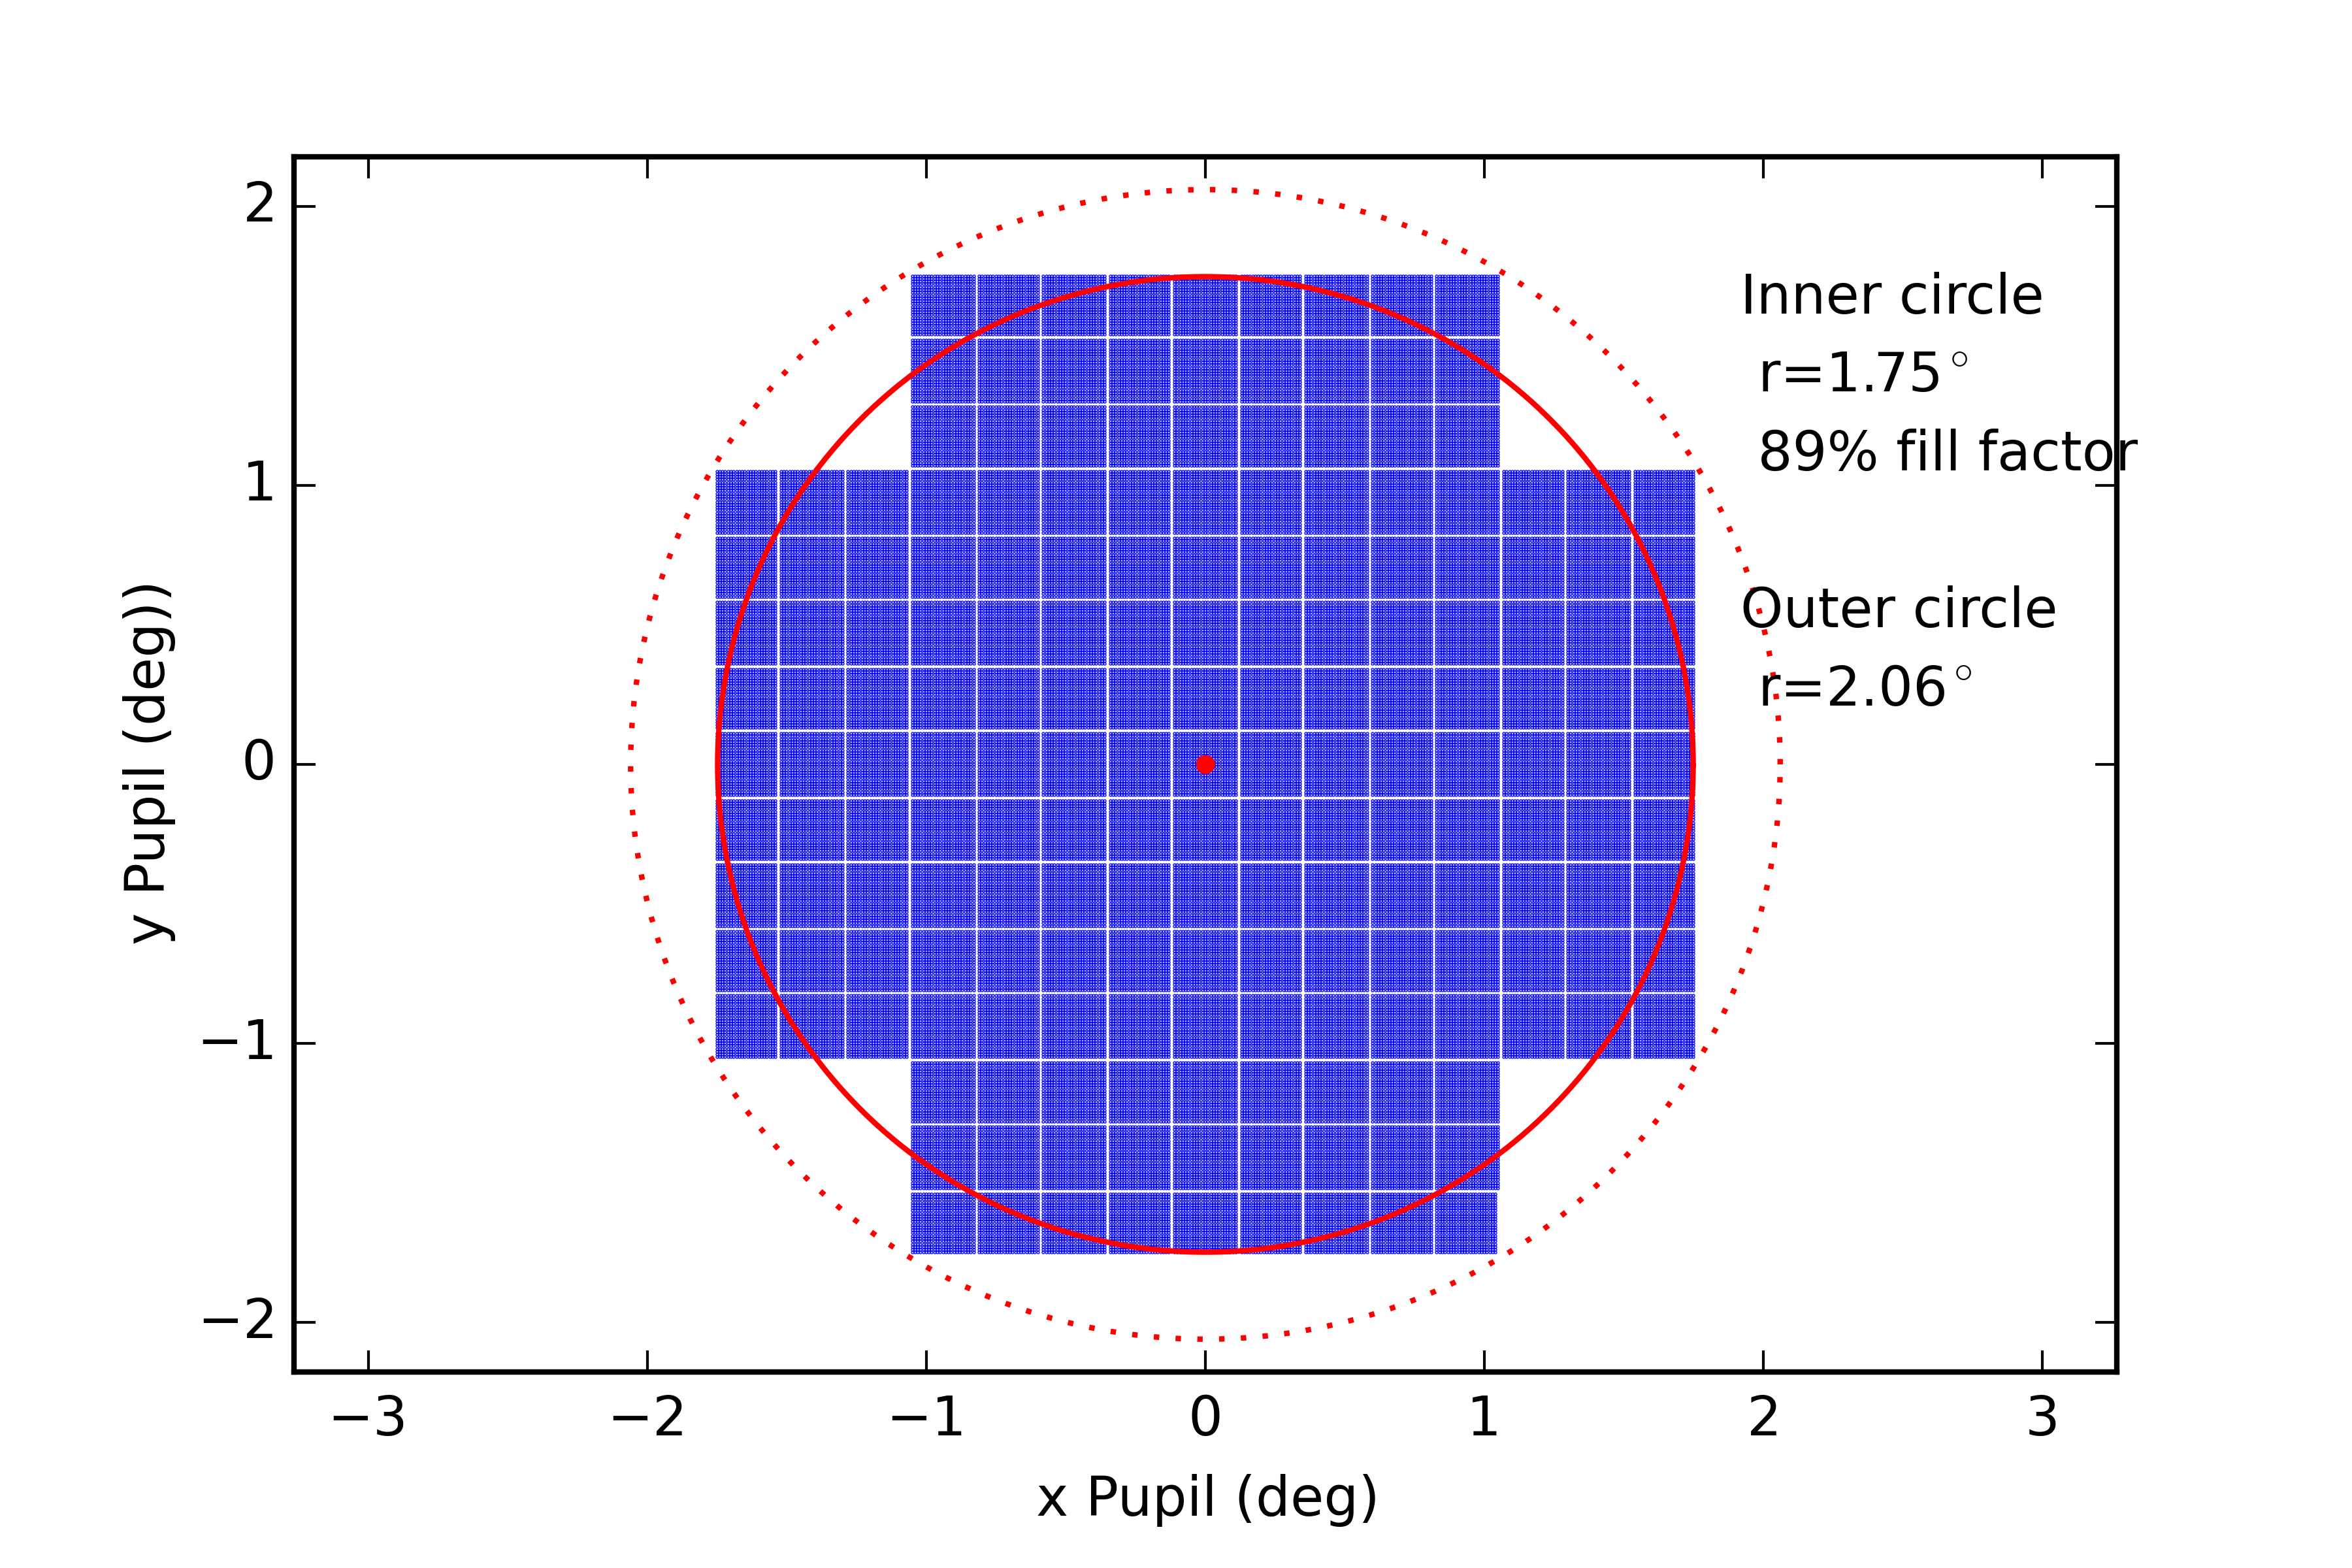
\includegraphics[width=0.9\linewidth]{focalplane}
\captionsetup{width=0.9\linewidth}
\caption{Layout of the LSST focal plane. The solid circle indicates
  the inscribed circular field of view (3.5$^\circ$ diameter). The
  plotted points indicate active silicon.\label{focalplane}}
\end{center}
\end{minipage}
\begin{minipage}{.5\textwidth}
\begin{center}
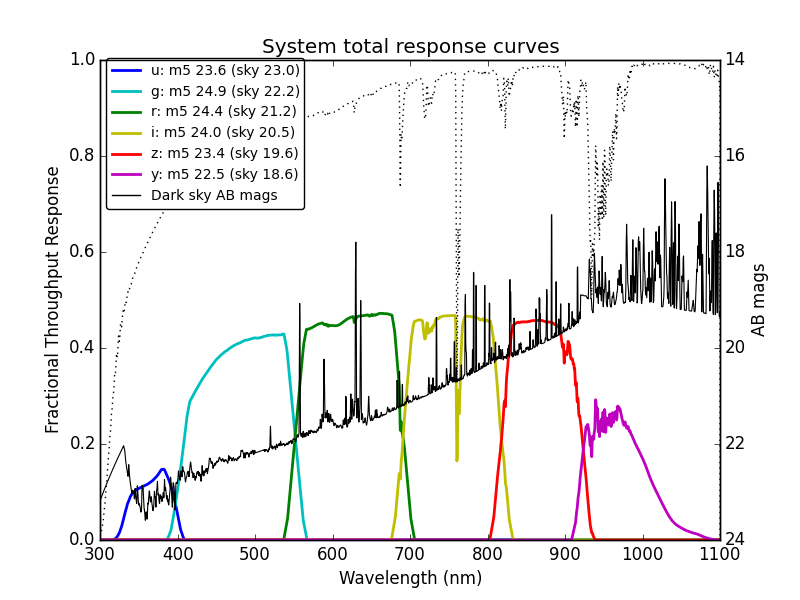
\includegraphics[width=0.9\linewidth]{throughputs}
\captionsetup{width=0.9\linewidth}
\caption{Expected LSST throughput response in $ugrizy$, including
  an X=1.2 atmospheric throughput curve (the dotted line). The
  expected dark sky brightness (in AB magnitudes) is also indicated,
  as the thin black line.\label{throughputs}}
\end{center}
\end{minipage}
\end{figure}


\section{LSST data management}

Over its lifetime, LSST will gather millions of images (on the order
of 2.5 million visits, consisting of a pair of back-to-back 15s
exposures). The information in these images must be processed into
measurements before it can be widely useful; turning these images into
queryable catalogs of detections and the associations of these
detections into astronomical sources (linking detections from each
visit with the related detections in other visits) will be done by the
LSST Data Management (DM) Pipeline.

The LSST DM pipeline will be entirely open source and publicly
available. The various repositories that make up the DM software stack
can currently be found on github at \url{http://github.com/lsst};
more information about the stack and instructions for installing the
LSST software stack can be found at \url{http://dm.lsst.org}.

LSST data products (images and catalogs) will be immediately publicly available to
institutions with data rights (currently: all US and Chilean
institutions and institutions which have signed an MOA with LSST
Corporation and their designees).  The details of these data products
are defined in detail in the LSST Data Products Definitions Document (DPDD)
\cite{LSST_DPDD}. In general, the catalogs can be
thought of as falling into three categories: Level 1, Level 2 and
Level 3.

Level 1 data products are created during nightly processing. The
images in each visit are combined to reject cosmic rays, then
subtracted from a template image created from previously acquired
imaging (typically 6 months to a year earlier). The detections
measured in each difference image correspond to transients, variables,
moving objects, and artifacts. These outputs will be run through
machine learning algorithms to help reject artifacts. The resulting
detections, along with relevant information from existing catalogs
such as identification of known variable stars or the location of
nearby background galaxies, will be released within 60 seconds of the
end of each visit as the LSST Alert stream.

In addition, these difference image catalogs (after removing known
variable stars) will be used to feed the LSST moving object processing
system (MOPS). MOPS will link detections from different visits within
a night into tracklets, combine these with tracklets from
other nights into tracks, and finally fit the tracks with orbits; it will also extend
known orbits with new detections of these objects. These moving object
catalogs will updated and released on a daily basis.

The Alert stream and the moving object catalogs (the linked orbits and
their individual detections) make up the Level 1 data products. It is
worth noting that moving objects which are measurably trailed in any
individual visit will be clearly identifiable in the Alert stream as
such; very fast-moving objects thus have an additional discovery
avenue via Alerts.

Level 2 data products are created during yearly data processing and
include a more precise level of calibration in photometry and
astrometry. During the yearly data processing, all existing images
will be re-processed using the most recent software release. These
data release catalogs will reach 10mmag absolute photometric accuracy
and 10mas absolute astrometric accuracy. The increased accuracy is
possible due to various algorithms that compute global solutions;
these are not run during nightly data processing.

Level 3 data products indicate data products resulting from
independently written (non-project) software, created using LSST data
access center compute resources. These data products will typically be
generated using extensions to the LSST DM software, and may or may be
publicly available depending on the user. Publicly available Level 3
data products which prove particularly useful could become fully
federated with LSST databases.

\section{The LSST survey strategy}

LSST's short exposure times, large mirror, and wide field of view combine
to create a telescope that can generate deep individual images of
moving objects without trailing (for objects moving slower than
$\approx1$ degree/day), cover the entire visible sky every few days in
multiple filters to capture variable and transient phenomena, and
gather observations of galaxies under a variety of conditions to very
deep limiting magnitudes over the course of ten years. The details of
the observing strategy determine how well the survey will do at
achieving each of these science goals.

It should be clear from the above that LSST is not a survey optimized
solely for discovering solar system objects, but that it has great
potential in this area.

lsst general survey strategy
not optimized for solar system objects, but obvious potential
working on plan to best balance science return among all goals
describe opsim and maf at a general level, as tools for simulations

\section{Survey strategy implications for moving objects}
extending capabilities of maf and simulation framework to moving
objects
calculate trailing losses and detection losses
include focal plane footprint
include m5 values from opsim and colors appropriate to sources
in particular (relevant for this symposium) we can look at PHA, NEO,
and MBA discovery and characterization
discovery rates with standard MOPS requirements/completeness
 various size distributions and effect on total number of objects
with extended MOPS requirements
with better MOPS requirements (and why we should continue to work on software)
how many objects can be detected as they trail
characterization - how many observations in general we obtain,
arclength
characterization example: detecting activity
characterization problem needing solution: determining colors
then colors + orbital elements -> families
and number of observations -> sparse lightcurve inversion
and colors + albedo relationship -> size distribution (better than
simple LF assumptions)
point users to repos (where?)

\section{Discovering moving objects with MOPS}
description of discovery requirements with current MOPS
requirements for MOPS to work:
 false positive rate (expected results, given DES/machine
 learning/etc) (driven harder here by other science areas)
   ccds within spec, crosstalk small, no optical ghosts, 
 capabilities of linking objects (results of previous experiments with
 prototypes)  improvements within MOPS
show number of chances to discovery an object and how many chances we
have as function of H 
ongoing work to understand limitations and capabilities of MOPS

\section{Conclusion}
timeline for lsst
briefly additional science cases
call for metrics and ways to make sure survey strategy is good for
moving objects



\begin{thebibliography}{}

\bibitem[LSST LSE-163 (2013)]{LSST_DPDD}
{Juric, M.} 2013, The LSST Data Products Definition Document, LSST LSE-163,
\url{http://www.lsst.org/content/data-products-definition-document}

\end{thebibliography}

%\begin{discussion}
%\end{discussion}

\end{document}
